\chapter{Sensori}
%\myChapter{Sensori}
\label{sec:sensori}
La seguente appendice ha l'obbiettivo di fornire chiarimenti ulteriori ai sensori valutati ed usti nel lavoro qui presentato.  

Principalmente in questo lavoro usiamo un giroscopio monoassiale. In letteratura, l'analisi della deambulazione viene 
affrontata mediante accelerometri, giroscopi e magnetometri. 
\section*{Accelerometro}
\label{sec:accelerometer}
Un accelerometro (vedi Figura \ref{fig:acc}) � un dispositivo elettromeccanico che misura le forze di accelerazione. Tali forze possono essere sia statiche, come la forza di gravit�, che dinamiche, causate muovendo l'accelerometro.\\
Gli usi immediati di un accelerometro sono 
\begin{itemize}
	\item misurando l'accelerazione statica delle forza di gravit�, si pu� calcolare l'angolo a cui � inclinato lo strumento.
	\item misurando l'accelerazione dinamica si pu� analizzare il modo in cui si sta muovendo il dispositivo  
\end{itemize}
Un applicazione industriale importante � l'airbag nelle macchine, la cui apertura scatta se l'accelerometro percepisce una brusca frenata.
Un'altra applicazione � quella implementata da Apple\tm nei suoi portatili per la protezione del disco rigido: se il portatile dovesse cadere mentre � acceso, l'accelerometro capta la caduta libera ed il sistema operativo viene terminato immediatamente in modo che la testina non sia sul disco. 

\begin{figure}
	\centering
	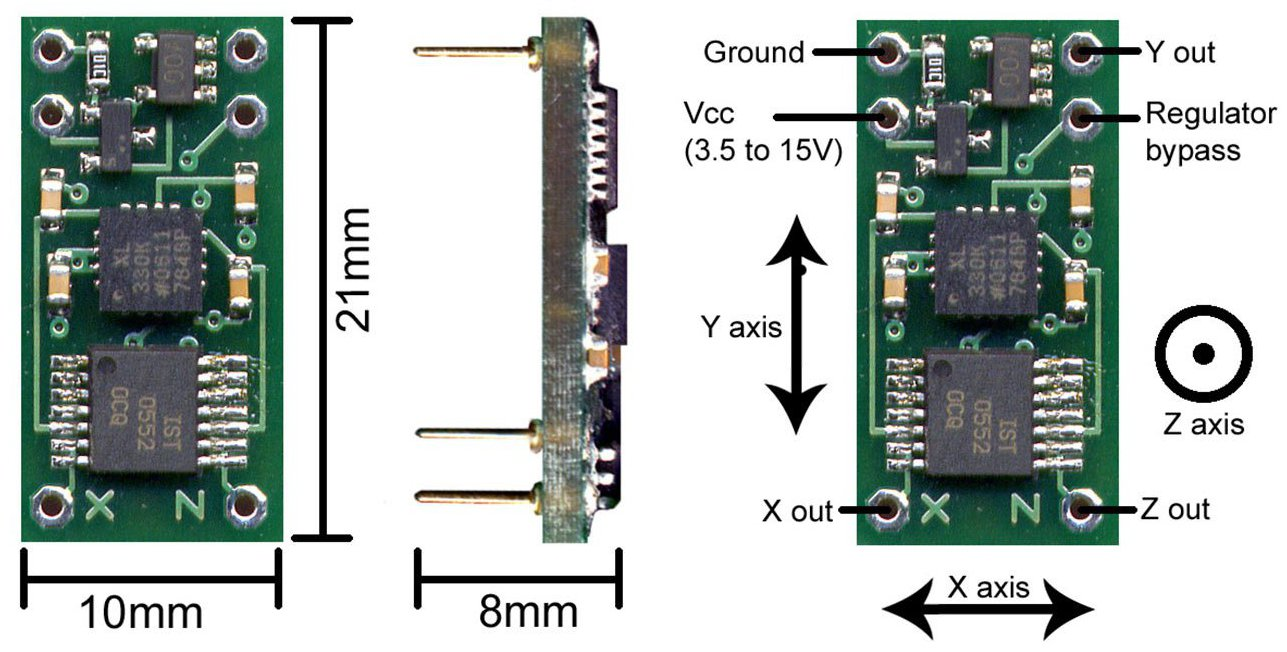
\includegraphics[width=1\textwidth]{imgs/acc_technical.jpg}
	\caption{ Accelerometro triassiale, cortesia di \url{http://www.dimensionengineering.com}}
	\label{fig:acc}
\end{figure}

\section*{Giroscopio}
\label{sec:gyroscope}
Il giroscopio � uno strumento per misurare l'accelerazione di rotazione (momento angolare) di un corpo. Vi sono diversi tipi di giroscopi, meccanici, a vibrazione, a fibre ottiche ecc..
Un disco rotante in assenza di torsione esterna, mantiene la direzione della sua rotazione 
 Quando viene applicata una torsione viene applicata al disco, ad angolo con il suo asse di rotazione, il disco ruota sul piano determinato dalle due assi (rotazione iniziale e torsione) nella direzione che va dall'asse di rotazione iniziale a quello della torsione.\\
Il tipo di giroscopio che usiamo in questo lavoro � il cosiddetto giroscopio piezoelettrico, o MEMS (\textit{Micro Electro Mechanical System}) o a vibrazione. Si basa sul principio di Coriolis: un oggetto che vibra, continua a vibrare sullo stesso piano se la struttura che lo sostiene � in rotazione. 
La misurazione della velocit� angolare avviene nel seguente modo: un elemento piezoelettrico (oggetto di forma tubolare) oscilla a causa di una rotazione, quindi viene misurata la forza di Coriolis sulla sezione longitudinale dell'elemento, dopo essere stata convertita in un voltaggio elettrico dallo stesso elemento piezoelettrico. 
 
\section*{Magnetometro}
\label{sec:magnetomerter}
Il Magnetometro � uno strumento che misura il campo magnetico. Questo pu� essere fatto in diversi modi. Il metodo pre elettronico, � quello inventato da Coulomb ed usa un ago magnetico sospeso.\\
Il metodo elettronico chiamato elettromagnetometro o Magnetometro \textit{Fluxgate} � basato sulla saturazione di materiali magnetici. Questi ha un centro in ferro, ed intorno ad esso due fili conduttori. Attraverso il primo filo fluisce corrente elettrica. Il ferro � un elemento magnetico, ma in condizioni normali gli assi magnetici sono orientati in direzioni casuali e la forza magnetica totale � prossima a zero. Nel momento in cui comincia a fluire corrente nel filo, gli assi si allineano e creano un campo magnetico percepibile come aumento del campo magnetico creato dalla corrente nel filo. La quantit� di forza magnetica che pu� produrre il ferro � limitata, il ferro giunge ad un livello di saturazione, dopo di che cambia bruscamente polarit�, al che giunge alla saturazione e cambia polarit� e cos� via. Questo processo induce corrente nel secondo filo che avvolge il ferro. Se la procedura avvenisse in un ambiente magneticamente neutrale il voltaggio nei due file dovrebbe combaciare, altrimenti vi sar� un dislivello proporzionale al campo magnetico di disturbo. L'intensit� del campo magnetico terrestre superficiale � circa 50,000 nano Tesla.  
\section*{IMU}
\label{sec:imu}
L'Unit� di Misura Inerziale (\textit{Inertial Measurement Unit}), � l'integrazione di pi� sensori. Questo fornisce le misure fatte dai sensori interni con eventuali correzioni sugli errori sistematici causati dalla temperatura interna dello strumento, umidit� ecc. Le IMU sono usate come sistemi di navigazione inerziali di aerei, missili. \\
La IMU che � stata usata nel lavoro presentato ha la seguente scheda di definizione: 

\begin{table}[htbp]
	\centering
\begin{tabular}{|m{4cm}|m{2.5cm}|m{5.3cm}|}
\hline
\multicolumn{3}{|c|}{IMU} \\ 
\hline
\textbf{Sensore}& \textbf{Intervallo di misurazione} & \textbf{Risoluzione} \\
\hline
\hline
\multirow{3}{*}{Accelerometro triassiale}& x[$\pm$1g-3g] & \multirow{3}{*}{[12-14 bit]}\\
&y[1.5g-2g/8g]&\\
&z[2g-16g]&\\
\hline
Giroscopio triassiale& [$\pm$2000-1600�/sec], & [12-16 bit]\\
\hline
Magnetometro triassiale& [$\pm$4 gauss], & 12 bit\\
\hline
Termometro & [-55-155�/C]& 12bit\\
\hline
\multicolumn{2}{|l|}{\textbf{Connettivit�}} & Bluetooth per le brevi distanze\\
%\multicolumn{3}{|r|}{Bluetooth per le brevi distanze}\\
\hline
\multicolumn{2}{|l|}{\textbf{Frequenza di campionamento}}&$\geq$ 300 Hz\\
%\multicolumn{1}{|r|}{$\geq$ 300 Hz}\\
\hline
\multicolumn{2}{|l|}{\textbf{Dimensioni strumento}}&60 $\times$ 30 $\times$ 40 mm\\		
\hline
%\multicolumn{1}{|r|}{60 $\times$ 30 $\times$ 40 mm} 	
\end{tabular}
	\caption{Scheda tecnica IMU}
	\label{tab:SchedaTecnicaIMU}
\end{table}



	